\section{Discussion}
\label{sec:4-discussion}
The maintenance scheduling process effectively solves a complex scheduling problem by
relying in multiple actors. Through the use of actors the scheduling process handles
uncertainty that is difficult to reason about in a single mathematical model. These 
uncertainties are solved through coordination. Each type of stakeholder in the process 
acts according to a  model each with different levels of aggregation and features where
each actor understands how to exploit his own model.
The discussion will be divided into three sections: 
\ref{sec:discussion:actors_and_integration} 
actors and integration;
\ref{sec:discussion:continuous_optimization} 
continuous optimization allows asynchronous optimization; 
and \ref{sec:discussion:future_research} future research.

\subsection{Actors \& Integration}
\label{sec:discussion:actors_and_integration}
Often in operation research the failure to reliably solve operational
problems in  industry are not due to the problems being computationally
intractable \cite{gendreauHandbookMetaheuristics2019} but a practical
problem of connecting data streams so that the solution approach continually
receives dynamic data to handle changes and then providing the resulting
solutions to the relevant actors (stakeholders) through a relevant interface
\cite{meignanReviewTaxonomyInteractive2015}. The actor-based approach proposed
in this paper makes integration easier by naturally encapsulating a model with a
reliable interface.

\subsection{Continuous Optimization}
\label{sec:discussion:continuous_optimization}
With actor-based metaheuristics, the optimization loop can run indefinitely,
optimizing based on the latest available information. This may seem like a
detail as you could argue that you should only ever optimize the schedule
when there is an explicit need for it, but consider the case when you start
adding more than two actors to a scheduling system, then there arises a need
to coordinate people temporally as each will have to run their optimizing
process one after another. This is depicted in figure~\ref{fig:discussion:hierarchical_model_setup}
where the output of one model is used as the input to the next one, leading
to the hierarchical model setup.

\begin{figure}[H]
	\usetikzlibrary{positioning}
\usetikzlibrary{arrows.meta}
\usetikzlibrary{bending}
\definecolor{red}{HTML}{8A3F3A}
\definecolor{yellow}{HTML}{E0BB3C}
\definecolor{blue}{HTML}{4569E0}
\definecolor{green}{HTML}{17E561}
\definecolor{other}{HTML}{6A939E}

% DTU Colors
\definecolor{dtu-corporate-red}{HTML}{990000}
\definecolor{dtu-white}{HTML}{ffffff}
\definecolor{dtu-black}{HTML}{000000}
\definecolor{dtu-blue}{HTML}{2F3EEA}
\definecolor{dtu-bright-green}{HTML}{1FD082}
\definecolor{dtu-navy-blue}{HTML}{030F4F}
\definecolor{dtu-yellow}{HTML}{F6D04D}
\definecolor{dtu-orange}{HTML}{FC7634}
\definecolor{dtu-pink}{HTML}{F7BBB1}
\definecolor{dtu-grey}{HTML}{DADADA}
\definecolor{dtu-red}{HTML}{E83F48}
\definecolor{dtu-green}{HTML}{008835}
\definecolor{dtu-purple}{HTML}{79238E}


\newlength{\basisb}
\setlength{\basisb}{0.4cm}

\centering
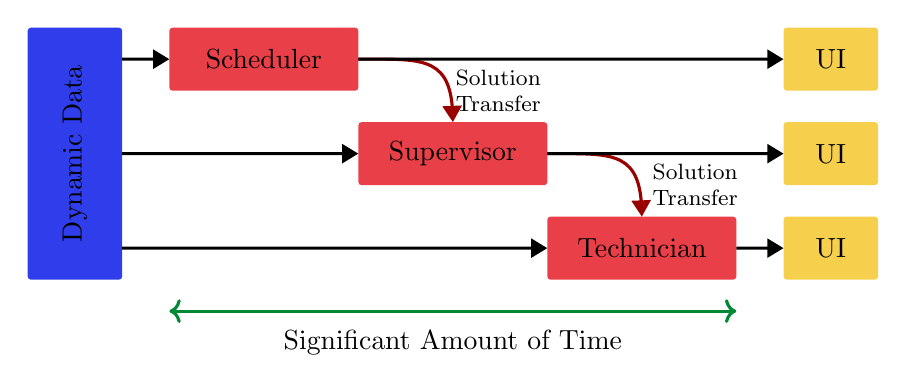
\begin{tikzpicture}[line width=0.0\basisb]
    \draw (2.0\basisb,4.0\basisb) 
		node[rotate=90, minimum height=3\basisb,fill=dtu-blue,minimum width=8\basisb,rounded corners=0.1\basisb] 
			(Dynamic Data) {Dynamic Data};

    \draw (8.0\basisb,7.0\basisb) 
		node[minimum height=2\basisb,fill=dtu-red,minimum width=6\basisb,rounded corners=0.1\basisb] 
			(Scheduler) {Scheduler};
    \draw (14.0\basisb,4.0\basisb) 
		node[minimum height=2\basisb,fill=dtu-red,minimum width=6\basisb,rounded corners=0.1\basisb] 
			(Supervisor) {Supervisor};
    \draw (20.0\basisb,1.0\basisb) 
		node[minimum height=2\basisb,fill=dtu-red,minimum width=6\basisb,rounded corners=0.1\basisb] 
			(Technician) {Technician};

    \draw (26.0\basisb,7.0\basisb) 
		node[minimum height=2\basisb,fill=dtu-yellow,minimum width=3\basisb,rounded corners=0.1\basisb] 
			(UserInterface1) {UI};
    \draw (26.0\basisb,4.0\basisb) 
		node[minimum height=2\basisb,fill=dtu-yellow,minimum width=3\basisb,rounded corners=0.1\basisb] 
			(UserInterface2) {UI};
    \draw (26.0\basisb,1.0\basisb) 
		node[minimum height=2\basisb,fill=dtu-yellow,minimum width=3\basisb,rounded corners=0.1\basisb] 
			(UserInterface3) {UI};

	\draw[<->, line width=0.1\basisb,color=dtu-green] (5.0\basisb, -1\basisb) -- (23.0\basisb, -1\basisb);
	\draw (14.0\basisb, -2.0\basisb) node {Significant Amount of Time};

	\draw[->,>=Triangle, thick, line width=0.1\basisb, color=dtu-corporate-red] (Scheduler) to[out=0, in=90,looseness=1.5]  (Supervisor);
	\draw[->,>=Triangle, thick, line width=0.1\basisb, color=dtu-corporate-red] (Supervisor) to[out=0, in=90,looseness=1.5] (Technician);
	\draw[->,>=Triangle, thick, line width=0.1\basisb] (Dynamic Data.south) ++(0\basisb,3.0\basisb) to[out=0, in=180,looseness=1.0] (Scheduler);
	\draw[->,>=Triangle, thick, line width=0.1\basisb] (Dynamic Data.south) to[out=0, in=180,looseness=1.0] (Supervisor);
	\draw[->,>=Triangle, thick, line width=0.1\basisb] (Dynamic Data.south) ++(0\basisb,-3.0\basisb) to[out=0, in=180,looseness=1.0] (Technician.west);
	\draw[<-,>=Triangle, thick, line width=0.1\basisb] (UserInterface1) to[out=180, in=0,looseness=1.0] (Scheduler);
	\draw[<-,>=Triangle, thick, line width=0.1\basisb] (UserInterface2) to[out=180, in=0,looseness=1.0] (Supervisor);
	\draw[<-,>=Triangle, thick, line width=0.1\basisb] (UserInterface3) to[out=180, in=0,looseness=1.0] (Technician);
	% \draw[<->, thick, line width=0.1\basisb] (Scheduler) -- (UserInterface);
	\begin{scope}[shift={(7,0)}] % Adjust shift to position the legend
    % Legend box
    % Legend lines and text
	    \draw[thick, line width=0.1\basisb] (-1.5,2.4) node[right, font=\footnotesize, align=center] {Solution\\Transfer};
	    \draw[thick, line width=0.1\basisb] (1.0,1.2) node[right, font=\footnotesize, align=center] {Solution\\Transfer};
	\end{scope}
\end{tikzpicture}

	\label{fig:discussion:hierarchical_model_setup}
	\caption{Effects of using hierarchical models setups in human-guided search metaheuristics.
	Due to the dependent nature of each metaheuristic it becomes crucial that the running of 
	the metaheuristics are well coordinated between the stakeholders.}
\end{figure}

In practice there are multiple problems with using a hierarchical setup.
Usually the biggest one is that the information and knowledge needed to 
execute a feasible schedule is usually found in the lower levels of the 
hierarchicy. The operational setting, where the
technicians are working, is usually so complex that it not feasible to 
centralize the knowledge that is required to create and execute a 
schedule. Figure~\ref{fig:discussion:asynchronous_setup}
shows the kind of non-hierarchical setup that an actor-based approach 
allows for.

\begin{figure}[H]
	\usetikzlibrary{positioning}
% \usetikzlibrary{arrows.meta}
\usetikzlibrary{bending}
\usetikzlibrary{backgrounds}
\definecolor{red}{HTML}{8A3F3A}
\definecolor{yellow}{HTML}{E0BB3C}
\definecolor{blue}{HTML}{4569E0}
\definecolor{green}{HTML}{17E561}
\definecolor{other}{HTML}{6A939E}

% DTU Colors
\definecolor{dtu-corporate-red}{HTML}{990000}
\definecolor{dtu-white}{HTML}{ffffff}
\definecolor{dtu-black}{HTML}{000000}
\definecolor{dtu-blue}{HTML}{2F3EEA}
\definecolor{dtu-bright-green}{HTML}{1FD082}
\definecolor{dtu-navy-blue}{HTML}{030F4F}
\definecolor{dtu-yellow}{HTML}{F6D04D}
\definecolor{dtu-orange}{HTML}{FC7634}
\definecolor{dtu-pink}{HTML}{F7BBB1}
\definecolor{dtu-grey}{HTML}{DADADA}
\definecolor{dtu-red}{HTML}{E83F48}
\definecolor{dtu-green}{HTML}{008835}
\definecolor{dtu-purple}{HTML}{79238E}


\newlength{\basisc}
\setlength{\basisc}{0.5cm}

\centering
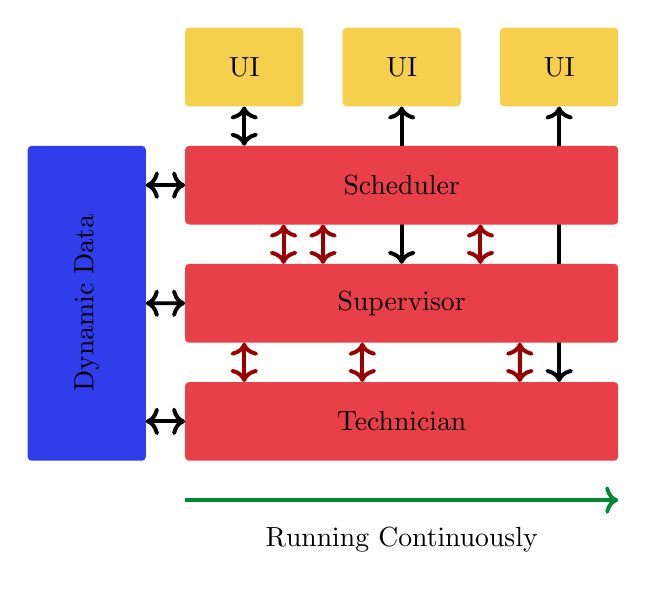
\begin{tikzpicture}[line width=0.0\basisc]
    \draw (4.0\basisc,4.0\basisc) 
		node[rotate=90, minimum height=3\basisc,fill=dtu-blue,minimum width=8\basisc,rounded corners=0.1\basisc] 
			(Dynamic Data) {Dynamic Data};

			

    \draw (8.0\basisc,10.0\basisc) 
		node[minimum height=2\basisc,fill=dtu-yellow,minimum width=3\basisc,rounded corners=0.1\basisc] 
			(UserInterface1) {UI};
    \draw (12.0\basisc,10.0\basisc) 
		node[minimum height=2\basisc,fill=dtu-yellow,minimum width=3\basisc,rounded corners=0.1\basisc] 
			(UserInterface2) {UI};
    \draw (16.0\basisc,10.0\basisc) 
		node[minimum height=2\basisc,fill=dtu-yellow,minimum width=3\basisc,rounded corners=0.1\basisc] 
			(UserInterface3) {UI};
    \draw (12.0\basisc,7.0\basisc) 
		node[minimum height=2\basisc,fill=dtu-red,minimum width=11\basisc,rounded corners=0.1\basisc] 
			(Scheduler) {Scheduler};
    \draw (12.0\basisc,4.0\basisc) 
		node[minimum height=2\basisc,fill=dtu-red,minimum width=11\basisc,rounded corners=0.1\basisc] 
			(Supervisor) {Supervisor};
    \draw (12.0\basisc,1.0\basisc) 
		node[minimum height=2\basisc,fill=dtu-red,minimum width=11\basisc,rounded corners=0.1\basisc] 
			(Technician) {Technician};


	\begin{pgfonlayer}{background}
		\draw[<->, thick, line width=0.1\basisc] (UserInterface1) to[out=-90, in=90,looseness=1.0] ++(0\basisc,-2.0\basisc)(Scheduler);
		\draw[<->, thick, line width=0.1\basisc] (UserInterface2) to[out=-90, in=90,looseness=1.0] (Supervisor);
		\draw[<->, thick, line width=0.1\basisc] (UserInterface3) to[out=-90, in=90,looseness=1.0] ++(0\basisc,-8.0\basisc)(Technician);

	\end{pgfonlayer}

	\draw[->, line width=0.1\basisc,color=dtu-green] (6.5\basisc, -1\basisc) -- (17.5\basisc, -1\basisc);
	\draw (12.0\basisc, -2.0\basisc) node {Running Continuously};

	\draw[<->, thick, line width=0.1\basisc, color=dtu-corporate-red] (Scheduler)++(-3\basisc, -1.0\basisc) to[out=-90, in=90,looseness=1.0]  ++(0\basisc, -1.0\basisc)(Supervisor);
	\draw[<->, thick, line width=0.1\basisc, color=dtu-corporate-red] (Scheduler)++(-2\basisc, -1.0\basisc) to[out=-90, in=90,looseness=1.0]  ++(0\basisc, -1.0\basisc)(Supervisor);
	\draw[<->, thick, line width=0.1\basisc, color=dtu-corporate-red] (Scheduler)++(2\basisc, -1.0\basisc) to[out=-90, in=90,looseness=1.0]  ++(0\basisc, -1.0\basisc)(Supervisor);

	\draw[<->, thick, line width=0.1\basisc, color=dtu-corporate-red] (Supervisor)++(-4\basisc, -1.0\basisc) to[out=-90, in=90,looseness=1.0] ++(0\basisc, -1.0\basisc)(Technician);
	\draw[<->, thick, line width=0.1\basisc, color=dtu-corporate-red] (Supervisor)++(-1\basisc, -1.0\basisc) to[out=-90, in=90,looseness=1.0] ++(0\basisc, -1.0\basisc)(Technician);
	\draw[<->, thick, line width=0.1\basisc, color=dtu-corporate-red] (Supervisor)++(3\basisc, -1.0\basisc) to[out=-90, in=90,looseness=1.0] ++(0\basisc, -1.0\basisc)(Technician);

	\draw[<->, thick, line width=0.1\basisc] (Dynamic Data.south) ++(0\basisc,3.0\basisc) to[out=0, in=180,looseness=1.0] (Scheduler);
	\draw[<->, thick, line width=0.1\basisc] (Dynamic Data.south) to[out=0, in=180,looseness=1.0] (Supervisor);
	\draw[<->, thick, line width=0.1\basisc] (Dynamic Data.south) ++(0\basisc,-3.0\basisc) to[out=0, in=180,looseness=1.0] (Technician.west);

	% \draw[<->, thick, line width=0.1\basisc] (Scheduler) -- (UserInterface);
\end{tikzpicture}

	\caption{Asynchronous model setup where each metaheuristic runs in perpetuity. In this setup
	there is no need to coordinate stakeholders to run the metaheuristics. Each actor in the 
	scheduling process will always have the solutions of the other stakeholder available to 
	him to guide his own search.}
	\label{fig:discussion:asynchronous_setup}
\end{figure}

When the optimization approach optimize continuously it enables tight
integration between the different model implementations. Instead of running
models to completion you simply handle changes in model parameters, model
solutions, user inputs, and in the dynamic data source as they occur opposed to
restarting the metaheuristics.

\subsection{Future Research}
% TODO 
By structuring system state changes as atomic pointer swaps, one can modularize
concurrency at each layer and ensure real-time synchronization across multiple
optimization levels.

% TODO 
By structuring system state changes as atomic pointer swaps, one can modularize
concurrency at each layer and ensure real-time synchronization across multiple
optimization levels.

% TODO 
Designing lock-free non-message-passing frameworks that handle
real-time atomic pointer updates across multiple actor layers. 

% TODO 
Exploring specialized hardware or runtime support for ultra-low-latency
coordination.

% TODO
Roadmap. Provide a short bullet list of concrete next steps—for instance, “(1)
building a robust pointer-swap concurrency library, (2) testing multi-level
coordination on standard benchmarks, (3) validating performance in real-time
scheduling applications.”

% TODO 
8. Future Research
While this paper details our initial development of an actor-based large
neighborhood search strategy, a range of exciting directions remain open. In
particular, the lock-free coordination mechanisms used here—implemented via
atomic pointer swaps—could be extended to n-level optimization problems where
multiple decision layers must operate asynchronously. Future research will delve
into both the theoretical aspects (e.g., convergence proofs for multi-level
actor systems) and practical considerations (e.g., specialized data structures
and memory-management schemes) to ensure real-time performance. Furthermore,
exploring hybrid models that integrate machine learning heuristics or advanced
decomposition methods can significantly broaden the applicability of our
actor-based framework. We anticipate that these developments, coupled with
extensive benchmarking on large-scale and time-critical scenarios, will provide
a robust foundation for solving increasingly complex optimization tasks.

\label{sec:discussion:future_research}
The future research direction is is to demonstrate that
the actor-based approach described here can be used to model and optimize 
multi-actor/multi-level scheduling processes. 
Figure~\ref{fig:ordinator-architecture}
shows a scheduling system architecture where each of the actors run an actor-based metaheuristic
and that each metaheuristic will share its solutions with the other
metaheuristics through atomic pointer swapping. Communicate with the end-user
through message passing, integrate with a persistent storage through mutex
locks, and the lifecycle of each of the metaheuristics will be controlled by
the orchestrator also through message passing. 

\begin{figure}[H]
	\centering
	\usetikzlibrary {positioning}

\definecolor{red}{HTML}{8A3F3A}
\definecolor{yellow}{HTML}{E0BB3C}
\definecolor{blue}{HTML}{4569E0}
\definecolor{green}{HTML}{17E561}
\definecolor{other}{HTML}{6A939E}

% DTU Colors
\definecolor{dtu-corporate-red}{HTML}{990000}
\definecolor{dtu-white}{HTML}{ffffff}
\definecolor{dtu-black}{HTML}{000000}
\definecolor{dtu-blue}{HTML}{2F3EEA}
\definecolor{dtu-bright-green}{HTML}{1FD082}
\definecolor{dtu-navy-blue}{HTML}{030F4F}
\definecolor{dtu-yellow}{HTML}{F6D04D}
\definecolor{dtu-orange}{HTML}{FC7634}
\definecolor{dtu-pink}{HTML}{F7BBB1}
\definecolor{dtu-grey}{HTML}{DADADA}
\definecolor{dtu-red}{HTML}{E83F48}
\definecolor{dtu-green}{HTML}{008835}
\definecolor{dtu-purple}{HTML}{79238E}


\newcommand{\ModelColor}{dtu-red}
\newcommand{\UserInterfaceColor}{dtu-yellow}
\newcommand{\PersistenceColor}{dtu-blue}
\newcommand{\PointerSwapColor}{dtu-green}
\newcommand{\OrchestratorColor}{dtu-bright-green}

\newcommand{\basisinput}{4cm}  % Default value if not set by /graph/basis

\pgfkeys{
	/graph/.is family, /graph,
	default/.style = {
		show_shared_pointer = false,
		show_orchestrator = false,
		show_persistence = false,
		show_user_interface = false,
		basisinput/.estore in = \basisinput,
	},
	show_shared_pointer/.estore in = \ShowSharedSolutionCommunication,
	show_orchestrator/.estore in = \ShowOrchestratorCommunication,
	show_persistence/.estore in = \ShowPersistenceCommunication,
	show_user_interface/.estore in = \ShowUserInterfaceCommunication,
	basisinput/.estore in = \basisinput,
}

\newlength{\basis}
\tikzset{
  basis/.code={\setlength{\basis}{\basisinput}}, % TikZ assignment code
  basis/.default=3cm,                   % Provide a default (\b@sis is undefined/unassigned)
  basis,                                % Set initial Value (\b@sis is defined/assigned)
}

\newcommand{\drawOrdinatorArchitecture}[1]{
	\pgfkeys{/graph, default, #1}
	\setlength{\basis}{\basisinput}
	\begin{tikzpicture}[scale=0.75, line width=0.05\basis]

		\ifthenelse{\equal{\ShowOrchestratorCommunication}{true}}{
			\draw[color=other,-, ultra thick] (Strategic) -- (Orchestrator);
			\draw[color=other,-, ultra thick] (Tactical) -- (Orchestrator);
			\draw[color=other,-, ultra thick] (Supervisor) -- (Orchestrator);
			\draw[color=other,-, ultra thick] (Operational_1) -- (Orchestrator);
			\draw[color=other,-, ultra thick] (Operational_2) -- (Orchestrator);
			\draw[color=other,-, ultra thick] (Operational_3) -- (Orchestrator);
		}{}
		% \draw[help lines] (0\basis, 0\basis) grid (10\basis, 8\basis);
		\draw (5\basis,4\basis) node[minimum height=5\basis,minimum width=7.0\basis,rounded corners=0.1\basis] {};

	    \draw[draw=black] (4.125\basis,4.0\basis) node[opacity=0.5, minimum height=3.5\basis,minimum width=6.25\basis,rounded corners=0.1\basis,fill=\PointerSwapColor] {} ;
	    \draw (2.5\basis,5.5\basis) node[minimum height=1\basis,minimum width=1\basis,fill=\ModelColor,rounded corners=0.1\basis] (Strategic) {Stra};
	    \draw (5.0\basis,4.0\basis) node[minimum height=1\basis,minimum width=1\basis,fill=\ModelColor,rounded corners=0.1\basis] (Supervisor) {Sup};
		\draw (7.5\basis,5.5\basis) node[minimum height=1\basis,minimum width=1\basis,fill=\ModelColor,rounded corners=0.1\basis] (Tactical) {Tac};

		\draw (2.5\basis,2.5\basis) node[minimum height=1\basis,minimum width=1\basis,fill=\ModelColor,rounded corners=0.1\basis] (Operational_1) {$O_{1}$};
		\draw (5.0\basis,2.5\basis) node[minimum height=1\basis,minimum width=1\basis,fill=\ModelColor,rounded corners=0.1\basis] (Operational_2) {$O_{2}$};
		\draw (7.5\basis,2.5\basis) node[minimum height=1\basis,minimum width=1\basis,fill=\ModelColor,rounded corners=0.1\basis,rounded corners=0.1\basis] (Operational_3) {$O_{3}$};
	
		\draw (Strategic) edge (Tactical);
		\draw (Strategic) edge (Tactical);
		\draw (5\basis,5.5\basis) edge (Supervisor);
		\draw (Supervisor) -- (2.5\basis,4.0\basis) -- (Operational_1);
		\draw (Supervisor) edge (Operational_2);
		\draw (Supervisor) -- (7.5\basis,4.0\basis) -- (Operational_3);
		\draw (5.0\basis,0.5\basis)   node[minimum height=1\basis,minimum width=5.0\basis,                fill=\PersistenceColor,rounded corners=0.1\basis] {persistence};
		\draw (5.0\basis,7.5\basis)   node[minimum height=1\basis,minimum width=5.0\basis,                fill=\OrchestratorColor,rounded corners=0.1\basis] (Orchestrator) {Orchestrator};
		\draw (0.5\basis,4.0\basis)   node[rotate=90, minimum height=1.0\basis, minimum width=3.5\basis,  fill=\PointerSwapColor,rounded corners=0.1\basis] {decision variables};
		\draw (9.5\basis,5.75\basis)  node[rotate=90, minimum height=1.0\basis, minimum width=1.0\basis,  fill=\UserInterfaceColor,rounded corners=0.1\basis] {UI};
		\draw (9.5\basis,4.0\basis)   node[rotate=90, minimum height=1.0\basis, minimum width=1.0\basis,  fill=\UserInterfaceColor,rounded corners=0.1\basis] {UI};
		\draw (9.5\basis,2.25\basis)  node[rotate=90, minimum height=1.0\basis, minimum width=1.0\basis,  fill=\UserInterfaceColor,rounded corners=0.1\basis] {UI};

		% Legend
		\begin{scope}[shift={(11.0\basis,5.7\basis)}]
			\node at (-0.25\basis,1\basis) [right] {};
			\draw[color=\OrchestratorColor,fill,rounded corners=0.1\basis] (0\basis,0.0\basis)   rectangle (0.5\basis, 0.5\basis);
			\node[anchor=west] at (0.5\basis, 0.25\basis) { Managing metaheuristic lifetimes };
			\draw[color=\PointerSwapColor,fill,rounded corners=0.1\basis] (0\basis,-1.0\basis)   rectangle(0.5\basis, -0.5\basis); 
			\node[anchor=west] at (0.5\basis, -0.75\basis) { Solution sharing (Atomic pointer swaps) };
			\draw[color=\ModelColor,fill,rounded corners=0.1\basis] (0\basis,-2.0\basis)         rectangle(0.5\basis, -1.5\basis); 
			\node[anchor=west] at (0.5\basis, -1.75\basis) { Metaheurics (Mathematical Models) };
			\draw[color=\PersistenceColor,fill,rounded corners=0.1\basis] (0\basis,-3.0\basis)   rectangle(0.5\basis, -2.5\basis); 
			\node[anchor=west] at (0.5\basis, -2.75\basis) { Data storage (Memory locks)};
			\draw[color=\UserInterfaceColor,fill,rounded corners=0.1\basis] (0\basis,-4.0\basis) rectangle(0.5\basis, -3.5\basis); 
			\node[anchor=west] at (0.5\basis, -3.75\basis) { Message passing (Memory channels) };

		\end{scope}
		\ifthenelse{\equal{\ShowSharedSolutionCommunication}{true}}{
			\draw[->, thick] (Strategic) -- (Orchestrator);
		}{}
		\ifthenelse{\equal{\ShowUserInterfaceCommunication}{true}}{
			\draw[->, thick] (Strategic) -- (Orchestrator);
		}{}
		\ifthenelse{\equal{\ShowPersistenceCommunication}{true}}{
			\draw[->, thick] (Strategic) -- (Orchestrator);
		}{}
		

	\end{tikzpicture}
}


	\drawOrdinatorArchitecture{basisinput=1cm}
	\caption{
		Overview of the scheduling process when modelled as actors. When LNS is encapsulated 
		is an actor it becomes possible to optimize parts of a large process individually instead of 
		optimizing the scheduling problem globally from a single model implementation.
	}
	\label{fig:ordinator-architecture}
\end{figure}

The next step in this research direction will be to model the remaining stakeholders as their own 
AbLNS metaheuristics, and then make them communicate together. Each exposing solutions to each 
other in real-time providing each other with high quality parameters.

\section{Conclusion}
Many current planning problems that industry faces are combinatorial by nature, 
and many combinatorial problems have to be solved continuously to make operations 
run efficiently. For operation research (OR) to be helpful in this process, the solution methods 
should be a minimally invasive in the workflow of the working stakeholders. 
The AbLNS solution approach detailed in this paper aligns
closely with both the known problems in operation research of the lack of integration and the issues of 
coordination in multi-stakeholder processes. For these reasons we argue that the
standard Operations Research approach of  first collecting data, then creating a
model and optimizing it and then finally providing the solution to the planners
in the company workflow, is not a sound approach in many situations.

We have here demonstrated AbLNS approach works in a practical setting,
maintenance scheduling at  Total Energies and we are convinced that this
approach, combining a number of smaller planning/optimization problems with
different actors/stakeholders responsible for their part of the overall
solution. This paper argues that making a system of numerous smaller  "quick
and dirty" models in an well thought out software architecture is much more
effective in practice than large integrated models.

The fundamental problem with the "older" paradigm is that optimizing across
actors/stakeholders is very difficult, leading the literature to prefer
integrated models instead of decomposing the model by each of the
processes that make up a business process such as maintenance scheduling.
This paper argues that this is mainly due to an outdated understanding of
software architecture that is available today in industry, but not acknowledged by broader the Operations Research
and Metaheuristic communities.
